\documentclass[journal,12pt,twocolumn]{IEEEtran}

\usepackage{setspace}
\usepackage{gensymb}
\singlespacing
\usepackage[cmex10]{amsmath}

\usepackage{amsthm}

\usepackage{mathrsfs}
\usepackage{txfonts}
\usepackage{amsmath}
\usepackage{stfloats}
\usepackage{float}
\usepackage{bm}
\usepackage{tikz}
\usepackage{pgfplots}
\usepackage{cite}
\usepackage{cases}
\usepackage{subfig}

\usepackage{longtable}
\usepackage{multirow}

\usepackage{enumitem}
\usepackage{mathtools}
\usepackage{steinmetz}
\usepackage{tikz}
\usepackage{circuitikz}
\usepackage{verbatim}
\usepackage{tfrupee}
\usepackage[breaklinks=true]{hyperref}
\usepackage{graphicx}
\usepackage{tkz-euclide}

\usetikzlibrary{calc,math}
\usepackage{listings}
    \usepackage{color}                                            %%
    \usepackage{array}                                            %%
    \usepackage{longtable}                                        %%
    \usepackage{calc}                                             %%
    \usepackage{multirow}                                         %%
    \usepackage{hhline}                                           %%
    \usepackage{ifthen}                                           %%
    \usepackage{lscape}
\usepackage{multicol}
\usepackage{chngcntr}
\usepackage{hyperref}
\hypersetup{
    colorlinks=true,
    linkcolor=blue,
    filecolor=blue,
    urlcolor=blue,
}
\DeclareMathOperator*{\Res}{Res}

\renewcommand\thesection{\arabic{section}}
\renewcommand\thesubsection{\thesection.\arabic{subsection}}
\renewcommand\thesubsubsection{\thesubsection.\arabic{subsubsection}}

\renewcommand\thesectiondis{\arabic{section}}
\renewcommand\thesubsectiondis{\thesectiondis.\arabic{subsection}}
\renewcommand\thesubsubsectiondis{\thesubsectiondis.\arabic{subsubsection}}


\hyphenation{op-tical net-works semi-conduc-tor}
\def\inputGnumericTable{}                                 %%

\lstset{
%language=C,
frame=single,
breaklines=true,
columns=fullflexible
}

\makeatletter
\setlength{\@fptop}{0pt}
\makeatother

\begin{document}


\newtheorem{theorem}{Theorem}[section]
\newtheorem{problem}{Problem}
\newtheorem{proposition}{Proposition}[section]
\newtheorem{lemma}{Lemma}[section]
\newtheorem{corollary}[theorem]{Corollary}
\newtheorem{example}{Example}[section]
\newtheorem{definition}[problem]{Definition}

\newcommand{\BEQA}{\begin{eqnarray}}
\newcommand{\EEQA}{\end{eqnarray}}
\newcommand{\define}{\stackrel{\triangle}{=}}
\bibliographystyle{IEEEtran}
\raggedbottom
\setlength{\parindent}{0pt}
\providecommand{\mbf}{\mathbf}
\providecommand{\pr}[1]{\ensuremath{\Pr\left(#1\right)}}
\providecommand{\qfunc}[1]{\ensuremath{Q\left(#1\right)}}
\providecommand{\sbrak}[1]{\ensuremath{{}\left[#1\right]}}
\providecommand{\lsbrak}[1]{\ensuremath{{}\left[#1\right.}}
\providecommand{\rsbrak}[1]{\ensuremath{{}\left.#1\right]}}
\providecommand{\brak}[1]{\ensuremath{\left(#1\right)}}
\providecommand{\lbrak}[1]{\ensuremath{\left(#1\right.}}
\providecommand{\rbrak}[1]{\ensuremath{\left.#1\right)}}
\providecommand{\cbrak}[1]{\ensuremath{\left\{#1\right\}}}
\providecommand{\lcbrak}[1]{\ensuremath{\left\{#1\right.}}
\providecommand{\rcbrak}[1]{\ensuremath{\left.#1\right\}}}
\theoremstyle{remark}
\newtheorem{rem}{Remark}
\newcommand{\sgn}{\mathop{\mathrm{sgn}}}
\providecommand{\abs}[1]{$\left\vert#1\right\vert$}
\providecommand{\res}[1]{\Res\displaylimits_{#1}}
\providecommand{\norm}[1]{\lVert#1\rVert}
%\providecommand{\norm}[1]{\lVert#1\rVert}
\providecommand{\mtx}[1]{\mathbf{#1}}
\providecommand{\mean}[1]{$E\left[ #1 \right]$}
\providecommand{\fourier}{\overset{\mathcal{F}}{ \rightleftharpoons}}
%\providecommand{\hilbert}{\overset{\mathcal{H}}{ \rightleftharpoons}}
\providecommand{\system}{\overset{\mathcal{H}}{ \longleftrightarrow}}
	%\newcommand{\solution}[2]{\textbf{Solution:}{#1}}
\newcommand{\solution}{\noindent \textbf{Solution: }}
\newcommand{\cosec}{\,\text{cosec}\,}
\providecommand{\dec}[2]{\ensuremath{\overset{#1}{\underset{#2}{\gtrless}}}}
\newcommand{\myvec}[1]{\ensuremath{\begin{pmatrix}#1\end{pmatrix}}}
\newcommand{\mydet}[1]{\ensuremath{\begin{vmatrix}#1\end{vmatrix}}}
\newcommand*{\permcomb}[4][0mu]{{{}^{#3}\mkern#1#2_{#4}}}
\newcommand*{\perm}[1][-3mu]{\permcomb[#1]{P}}
\newcommand*{\comb}[1][-1mu]{\permcomb[#1]{C}}
\numberwithin{equation}{subsection}
\makeatletter
\@addtoreset{figure}{problem}
\makeatother
\let\StandardTheFigure\thefigure
\let\vec\mathbf
\renewcommand{\thefigure}{\theproblem}
\def\putbox#1#2#3{\makebox[0in][l]{\makebox[#1][l]{}\raisebox{\baselineskip}[0in][0in]{\raisebox{#2}[0in][0in]{#3}}}}
     \def\rightbox#1{\makebox[0in][r]{#1}}
     \def\centbox#1{\makebox[0in]{#1}}
     \def\topbox#1{\raisebox{-\baselineskip}[0in][0in]{#1}}
     \def\midbox#1{\raisebox{-0.5\baselineskip}[0in][0in]{#1}}
\vspace{3cm}
\title{Assignment 4}
\author{Perambuduri Srikaran - AI20BTECH11018}
\maketitle
\newpage
\bigskip
\renewcommand{\thefigure}{\theenumi}
\renewcommand{\thetable}{\theenumi}
Download all python codes from
\begin{lstlisting}
https://github.com/srikaran-p/EE3900/tree/main/Assignment4/codes
\end{lstlisting}
Download all latex codes from
\begin{lstlisting}
https://github.com/srikaran-p/EE3900/tree/main/Assignment4
\end{lstlisting}
\section*{Problem}
(Linear Forms Q2.20) Find the equation of the line through the point $\myvec{0 \\ 2}$ making an angle $\frac{2\pi}{3}$ with the positive x-axis. Also, find the equation of the line parallel to it and crossing the y-axis at a distance of 2 units below the origin.
\section*{Solution}
The direction vector of the line is $\myvec{1 \\ -\sqrt{3}}$. The normal vector $\vec{n}$
\begin{align}
    \vec{n} &= \myvec{0 & -1 \\ 1 & 0}\myvec{1 \\ -\sqrt{3}}\\
    &= \myvec{\sqrt{3} \\ 1}
\end{align}
Let $\vec{P}$ be $\myvec{0 \\ 2}$. The equation of line in terms of normal vector
\begin{align}
    \vec{n}^T(\vec{x} - \vec{P}) &= 0\\
    \myvec{\sqrt{3} & 1}\vec{x} &= \myvec{\sqrt{3} & 1}\vec{P}\\
    \myvec{\sqrt{3} & 1}\vec{x} &= \myvec{\sqrt{3} & 1}\myvec{0 \\ 2}\\
    \myvec{\sqrt{3} & 1}\vec{x} &= 2
\end{align}
The standard basis vectors in 2D plane are
\begin{align}
    \vec{e_1} = \myvec{1 \\ 0}\\
    \vec{e_2} = \myvec{0 \\ 1}
\end{align}
The point which crosses the y-axis at a distance of 2 units below the origin
\begin{align}
    \vec{Q} &= \frac{-2\vec{e_2}}{\vec{n}^T\vec{e_2}}\\
    &= \frac{-2}{1}\vec{e_2}\\
    &= \myvec{0 \\ -2}
\end{align}
The equation of line which passes through $\vec{Q}$
\begin{align}
    \vec{n}^T(\vec{x} - \vec{Q}) &= 0\\
    \myvec{\sqrt{3} & 1}\vec{x} &= \myvec{\sqrt{3} & 1}\vec{Q}\\
    \myvec{\sqrt{3} & 1}\vec{x} &= \myvec{\sqrt{3} & 1}\myvec{0 \\ -2}\\
    \myvec{\sqrt{3} & 1}\vec{x} &= -2
\end{align}
\begin{figure}[htp]
    \centering
    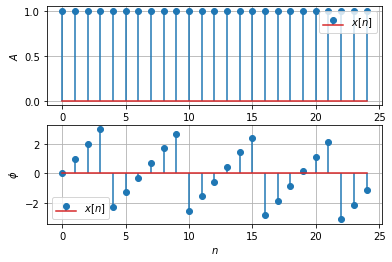
\includegraphics[width=\columnwidth]{Fig1.png}
    \caption{Plot of the given points and lines}
    \label{fig:plot}
\end{figure}
\end{document}
